
\section{Average number of generations until equilibrium}
There are numerous parameters that may affect the average number of generations until  equilibrium is reached. We chose to focus on the effect of the Happiness Rule(HR) on the average number of generations. For each HR ranging from 0 to 1 with increment 0.01, we ran 500 simulations and calculated the average, maximal and minimal generations it took to reach equilibrium. The results are shown in figure \ref{fig:avegen}.\\
\\
From figure \ref{fig:avegen}, we conclude that the average number of generations (blue graph) is increasing with the Happiness Rule, which is to be expected since a higher HR implies a higher need for neighbours of the same type, and thus a lower probability that a selected individual is happy, making it more likely that he/she will move. We also note that starting at a HR of aproximately 0.7, the average number of generations appears to be nearly constant. This can be explained noting that the required number of neighbours will practically be the same. For example, if the HR were 0.8, a person with 3, 5 or 8 neighbours would require respectively 3, 5 or at least 7 of the same type. This requirement hardly changes if a HR of 0.9 is applied. The same argument explains why the average number of generations is constant at very low HR or if we raise the HR with a sufficiently small amount like 0.01.\\
\\
\begin{figure}[h!]
    \centering
    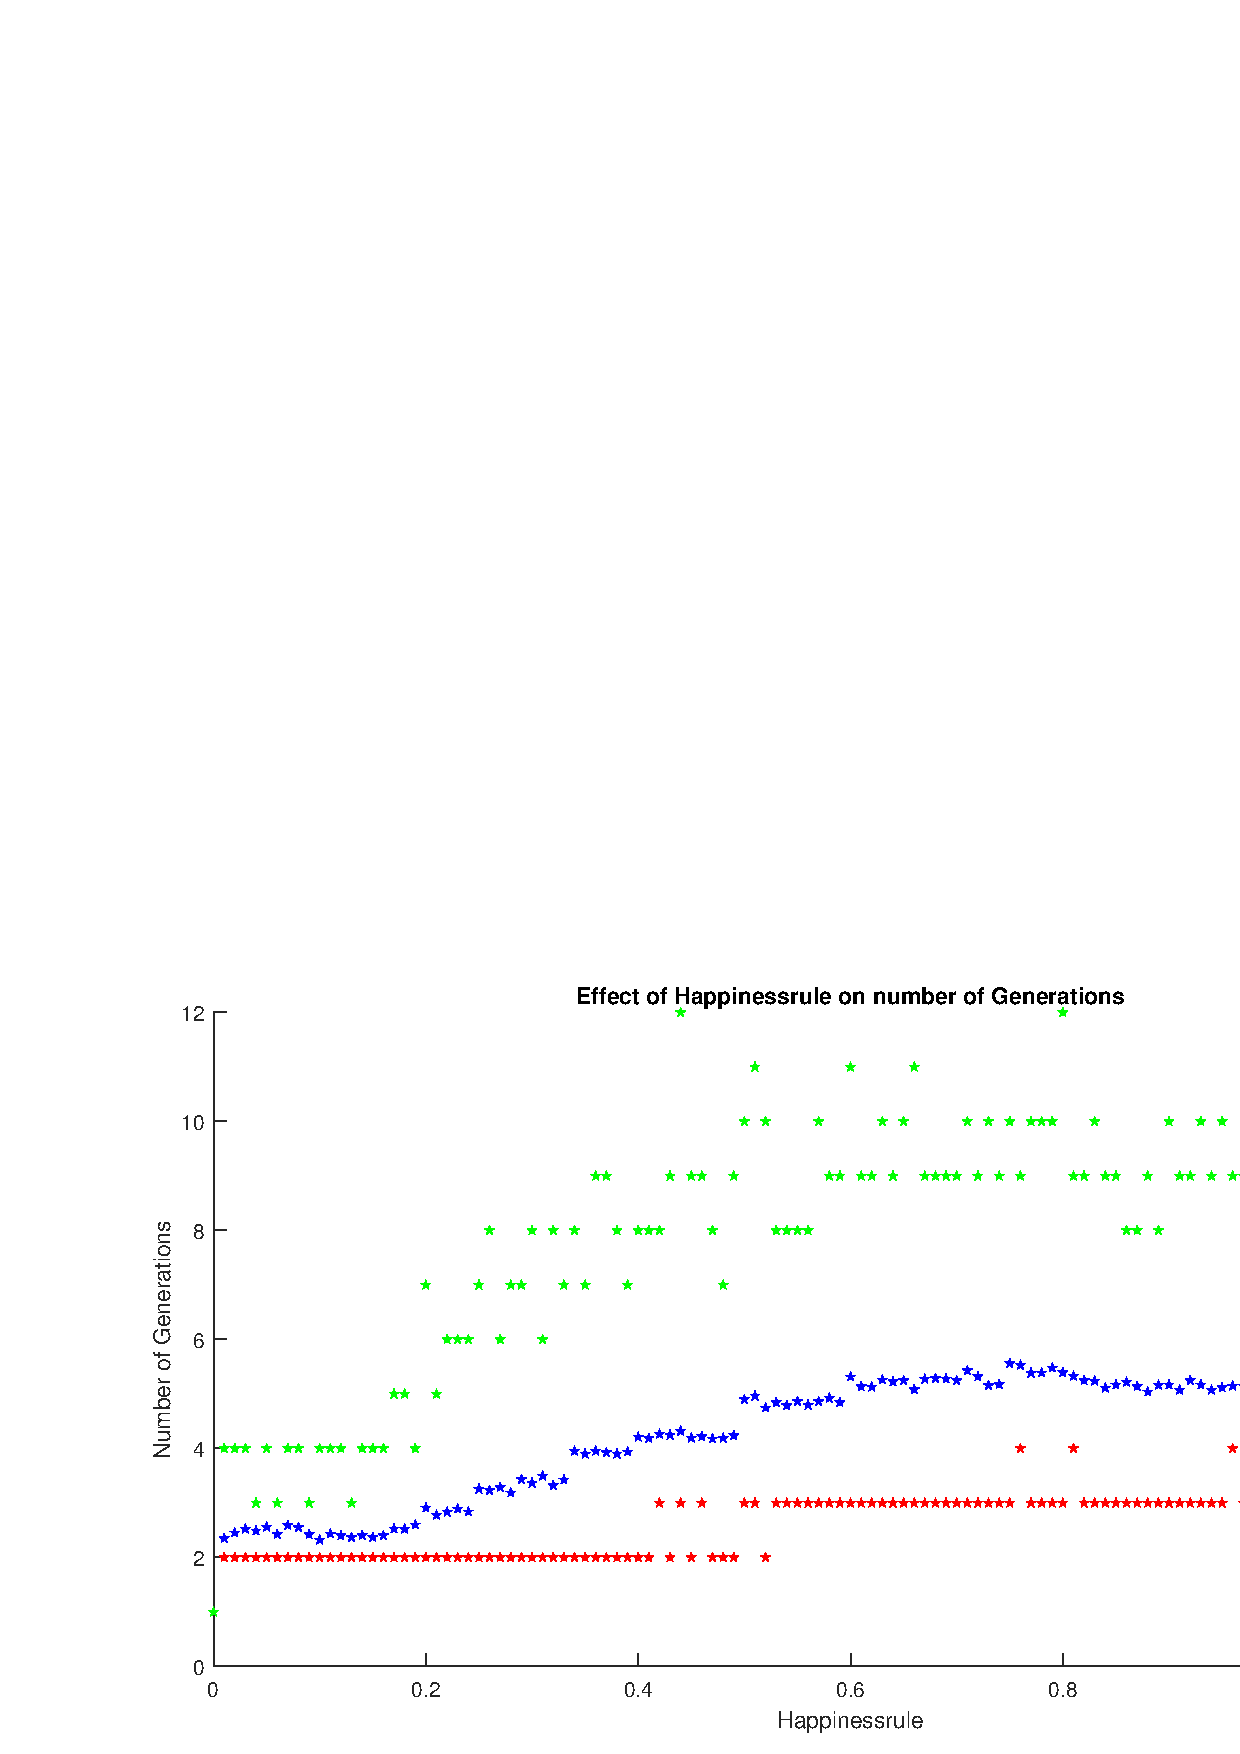
\includegraphics[width=0.9\textwidth]{happinessregel_aantgen_2.pdf}
    \caption{Effect of the happiness rule on the number of generations until reaching equilibrium. The green graph represents the maximal number of generations, the blue graph the average number of generations and the red graph displays the minimal number of generations}
    \label{fig:avegen}
\end{figure}
\\
As is one of the research questions, it is also interesting to know how the random variable $Y$, which we denote as the number of generations it takes to reach the equilibrium, is distributed. Since $Y$ depends on the position of each individual, whose positions in turn depend on other individuals, the probability distribution of $Y$ might be complicated. Therefore, we approximate the distribution of $Y$ with a histogram (figure \ref{fig:histogram}) of bin size 1, which is justifiable since $Y$ only takes integer values. Furthermore, in order to study the effect of the HR on the distribution of $Y$, we made histograms with Hapiness Rules of 1/4, 1/3, 1/2 and 1.  We believe that the histograms are a good model for the distribution of $Y$, as by the law of large numbers, the histogram will converge to the actual distribution for large numbers of simulations, and we may consider 10000 as a large number.\\
\\
 
\begin{figure}[H]
	
    \centering
    \begin{subfigure}{0.4\textwidth}
        \includegraphics[width=\textwidth]{GenormHistogramAantalgen4}
        \caption{10000 simulations of number of generations until equilibrium with HR 1/4}
        \label{fig:gull}
    \end{subfigure}
    ~ %add desired spacing between images, e. g. ~, \quad, \qquad, \hfill etc. 
      %(or a blank line to force the subfigure onto a new line)
    \begin{subfigure}{0.4\textwidth}
        \includegraphics[width=\textwidth]{GenormHistogramAantalgen}
        \caption{10000 simulations of number of generations until equilibrium with HR 1/3}
        \label{fig:tiger}
    \end{subfigure}
    ~ %add desired spacing between images, e. g. ~, \quad, \qquad, \hfill etc. 
    %(or a blank line to force the subfigure onto a new line)
    \begin{subfigure}{0.4\textwidth}
        \includegraphics[width=\textwidth]{GenormHistogramAantalgen2}
        \caption{10000 simulations of number of generations until equilibrium with HR 1/2}
        \label{minimal happiness 1}
    \end{subfigure}
    \begin{subfigure}{0.4\textwidth}
        \includegraphics[width=\textwidth]{GenormHistogramAantalgen1}
        \caption{10000 simulations of number of generations until equilibrium with HR 1}
        \label{minimal happiness 2}
    \end{subfigure}
    \caption{The probability distribution of $Y$ (the number of generations until reaching the equilibrium) is approximated with a histogram of bin size 1. For each HR(1/4, 1/3, 1/2 and 1), 10000 simulations were ran.}\label{fig:histogram}
\end{figure}

From figure \ref{fig:histogram}, we note that the distribution of $Y$ is fairly similar to the binomial distribution. We refrain from concluding that it is binomially distributed  however, as increasing the amount of simulations does not result in a more symmetrical distribution. It is up to this point unclear to us how \(Y\) is distributed.\\
\\
A fact worth noting, is that both the mean and the variance increase with the happiness rule. In line with the following section, the mean remains fairly low, while the number of generations tend to be fairly spread.\\
\textbf{Partial explanation.} While not immediately intuitive, the relatively small mean cannot be immediately explained. We do have an explanation for the relatively high frequency of the large number of generations however: If, after a few generations, equilibrium is not reached, the chance to move to a proper location decreases. Further details of this are provided in the following section. Thus, reaching equilibrium costs a fairly great amount of time.